\documentclass[10pt,letterpaper]{article}
\usepackage[T1]{fontenc}
\usepackage{lmodern}
\usepackage[margin=0.82in,headheight=14pt,footskip=24pt]{geometry}
\usepackage{microtype}
\usepackage{booktabs,tabularx,array,graphicx,xcolor,fancyhdr}
\usepackage[colorlinks=true,allcolors=blue!55!black,
  pdfauthor={Yuelin Li and Xiaoyu Chen},
  pdftitle={AffectNet-style Expression Classification on FER2013}]{hyperref}

\definecolor{ink}{HTML}{18283B}
\definecolor{accent}{HTML}{154D67}
\definecolor{muted}{HTML}{486175}
\setlength{\parindent}{0pt}
\setlength{\parskip}{5pt}
\setlength{\tabcolsep}{4pt}
\renewcommand{\arraystretch}{1.16}
\newcolumntype{Y}{>{\raggedright\arraybackslash}X}
\newcommand{\eyebrow}[1]{{\small\sffamily\bfseries\color{accent}#1}\par}
\newcommand{\note}[1]{{\small\color{muted}#1\par}}
\newcommand{\term}[1]{\textbf{#1}}
\newcommand{\metric}[1]{#1\%}
\newcommand{\pp}[1]{#1\,pp}
\newcommand{\sizepx}[1]{#1\ensuremath{\times}#1}

\pagestyle{fancy}
\fancyhf{}
\fancyhead[L]{\small\sffamily\color{muted}AffectNet2013 Workshop}
\fancyhead[R]{\small\sffamily\color{muted}FER2013 images \textbar{} FER+ labels}
\fancyfoot[R]{\small\sffamily\color{muted}\thepage}
\renewcommand{\headrulewidth}{0.35pt}
\setlength{\emergencystretch}{2em}
\raggedbottom

\begin{document}

\eyebrow{EXPERIMENT REPORT}
\vspace{3pt}
{\fontsize{27}{31}\selectfont\sffamily\bfseries\color{ink}
AffectNet-style expression\\classification on FER2013\par}
\vspace{5pt}
{\large\color{muted}Six training runs and one ensemble on eight FER+ classes\par}
\vspace{6pt}
{\normalsize\sffamily\bfseries\color{ink}Yuelin Li and Xiaoyu Chen\par}
\vspace{8pt}

\section{Data and protocol}

The workshop adapts the \href{https://arxiv.org/abs/1708.03985}{AffectNet classification baseline} to the original FER2013 images with \href{https://github.com/microsoft/FERPlus}{Microsoft FER+ annotations}. The source CSV matches the original Kaggle checksum. Filtering removed images, ties, and examples dominated by unknown or non-face votes yields 26,940 training, 3,396 validation, and 3,376 test examples from the original Training, PublicTest, and PrivateTest partitions. The eight classes are neutral, happy, surprise, sad, angry, disgust, fear, and contempt. FER2013 supplies expression labels only.

All runs use seed 42, AdamW, a OneCycle schedule, inverse-square-root class weighting, data augmentation, and horizontal-flip test-time augmentation. Validation macro-F1 selects each checkpoint. Macro-F1 gives equal weight to each class, including scarce classes such as disgust and contempt. Accuracy measures the fraction of correct predictions. Each configuration was run once.

\section{Training configurations}

{\small
\begin{tabularx}{\textwidth}{@{}lYlYrr@{}}
\toprule
Exercise & Model & Input & Initialization & Epochs & Peak LR\\
\midrule
1  & ResNet-18 baseline      & \sizepx{128} & ImageNet & 25 & 0.0005\\
2  & Native ResNet-18        & \sizepx{48}  & ImageNet & 25 & 0.0005\\
3  & Tuned ResNet-18         & \sizepx{128} & ImageNet & 55 & 0.0003\\
4a & ResNet-18 from scratch  & \sizepx{128} & Random   & 25 & 0.0005\\
4b & AlexNet                 & \sizepx{128} & ImageNet & 30 & 0.0005\\
4d & Inception-ResNet-v1     & \sizepx{160} & VGGFace2 & 30 & 0.0002\\
\bottomrule
\end{tabularx}\par}

\term{Native resolution.} A \sizepx{3} stride-1 convolution uses the center of the pretrained \sizepx{7} filters. A \sizepx{2} pool sends a \sizepx{24} map into the first residual stage. The standard stem would reduce a \sizepx{48} input to \sizepx{12} before that stage. The native variant keeps a \sizepx{3} map before global pooling.

\term{Longer schedule.} The tuned run uses an exponential moving average (EMA) of the weights with decay 0.995 per batch and learns from \href{https://arxiv.org/abs/1608.01041}{FER+ annotator vote shares}. Label smoothing drops from 0.10 to 0.02 because the votes already express uncertainty. All runs use the same hard targets for validation and test scoring.

\term{Face recognition pretraining.} \href{https://github.com/timesler/facenet-pytorch}{FaceNet} starts from \href{https://arxiv.org/abs/1710.08092}{VGGFace2} identity weights, replaces the identity classifier with an eight-class head, and fine-tunes the full network with FaceNet's input standardization. Compared with the baseline, it also changes the backbone, resolution, and learning rate.

\newpage
\section{Test results}

Each model was evaluated on the same 3,376 private-test examples. Deltas are in percentage points relative to the baseline.

{\small
\begin{tabularx}{\textwidth}{@{}lYrrrrrr@{}}
\toprule
& & Best & Val & Test & Test & $\Delta$ & $\Delta$\\
Exercise & Model & epoch & macro-F1 & macro-F1 & accuracy & macro-F1 & accuracy\\
\midrule
1  & ResNet-18 baseline      & 21 & 76.37\% & 72.32\% & 85.49\% & 0.00 & 0.00\\
2  & Native \sizepx{48}      & 13 & 75.05\% & 70.89\% & 83.23\% & $-1.43$ & $-2.25$\\
3  & Longer schedule and EMA & 16 & 75.32\% & 69.50\% & 84.57\% & $-2.82$ & $-0.92$\\
3b & Equal-weight ensemble   & -- & \textbf{77.24\%} & 73.29\% & \textbf{87.23\%} & $+0.97$ & \textbf{+1.75}\\
4a & ResNet-18 from scratch  & 23 & 72.76\% & 67.78\% & 82.49\% & $-4.54$ & $-2.99$\\
4b & AlexNet                 & 26 & 69.28\% & 68.24\% & 82.32\% & $-4.08$ & $-3.17$\\
4d & VGGFace2 FaceNet        & 25 & 76.50\% & \textbf{73.99\%} & 86.49\% & \textbf{+1.67} & $+1.01$\\
\bottomrule
\end{tabularx}\par}

\subsection*{Resolution and class imbalance}

Baseline F1 was \metric{94.9} for happy, \metric{45.0} for disgust, and \metric{48.0} for contempt. The test set has only 22 disgust and 26 contempt examples, so a few predictions can noticeably change macro-F1. The native run improved disgust F1 to \metric{47.8} and contempt F1 to \metric{51.3}, while fear F1 dropped from \metric{62.1} to \metric{57.0}. The experiment changes the input and stem together. Upsampling to \sizepx{128} gives pretrained filters a denser grid while interpolating the existing pixels.

\subsection*{Accuracy improvement}

For the 55-epoch recipe, validation macro-F1 peaked at epoch 16 while training loss continued to fall. Disgust recall rose from \metric{40.9} to \metric{59.1}, but precision fell from \metric{50.0} to \metric{25.0}. The changes in targets and smoothing affect the scale of the reported loss.

The second attempt averages the class probabilities from the baseline, the native-resolution ResNet-18, and FaceNet. The members use different input processing and pretraining, and averaging can temper confident errors when members disagree. This ensemble reuses existing checkpoints and increases test accuracy by \pp{1.75} and macro-F1 by \pp{0.97}.

\subsection*{Pretraining}

ImageNet initialization improved ResNet-18 test macro-F1 by \pp{4.54} and accuracy by \pp{2.99} under the same 25-epoch schedule. At epoch 5, validation macro-F1 was \metric{67.7} with ImageNet weights and \metric{48.4} from scratch.

FaceNet achieved the highest test macro-F1. It gained \pp{1.67} macro-F1 and \pp{1.01} accuracy over the baseline, \pp{6.21} and \pp{4.00} over random initialization, and \pp{5.75} and \pp{4.18} over AlexNet. Relative to the baseline, disgust and fear F1 rose to \metric{51.3} and \metric{65.1}, while contempt F1 fell to \metric{46.5}.

\newpage
\section{ResNet-18 versus AlexNet during training}

\begin{center}
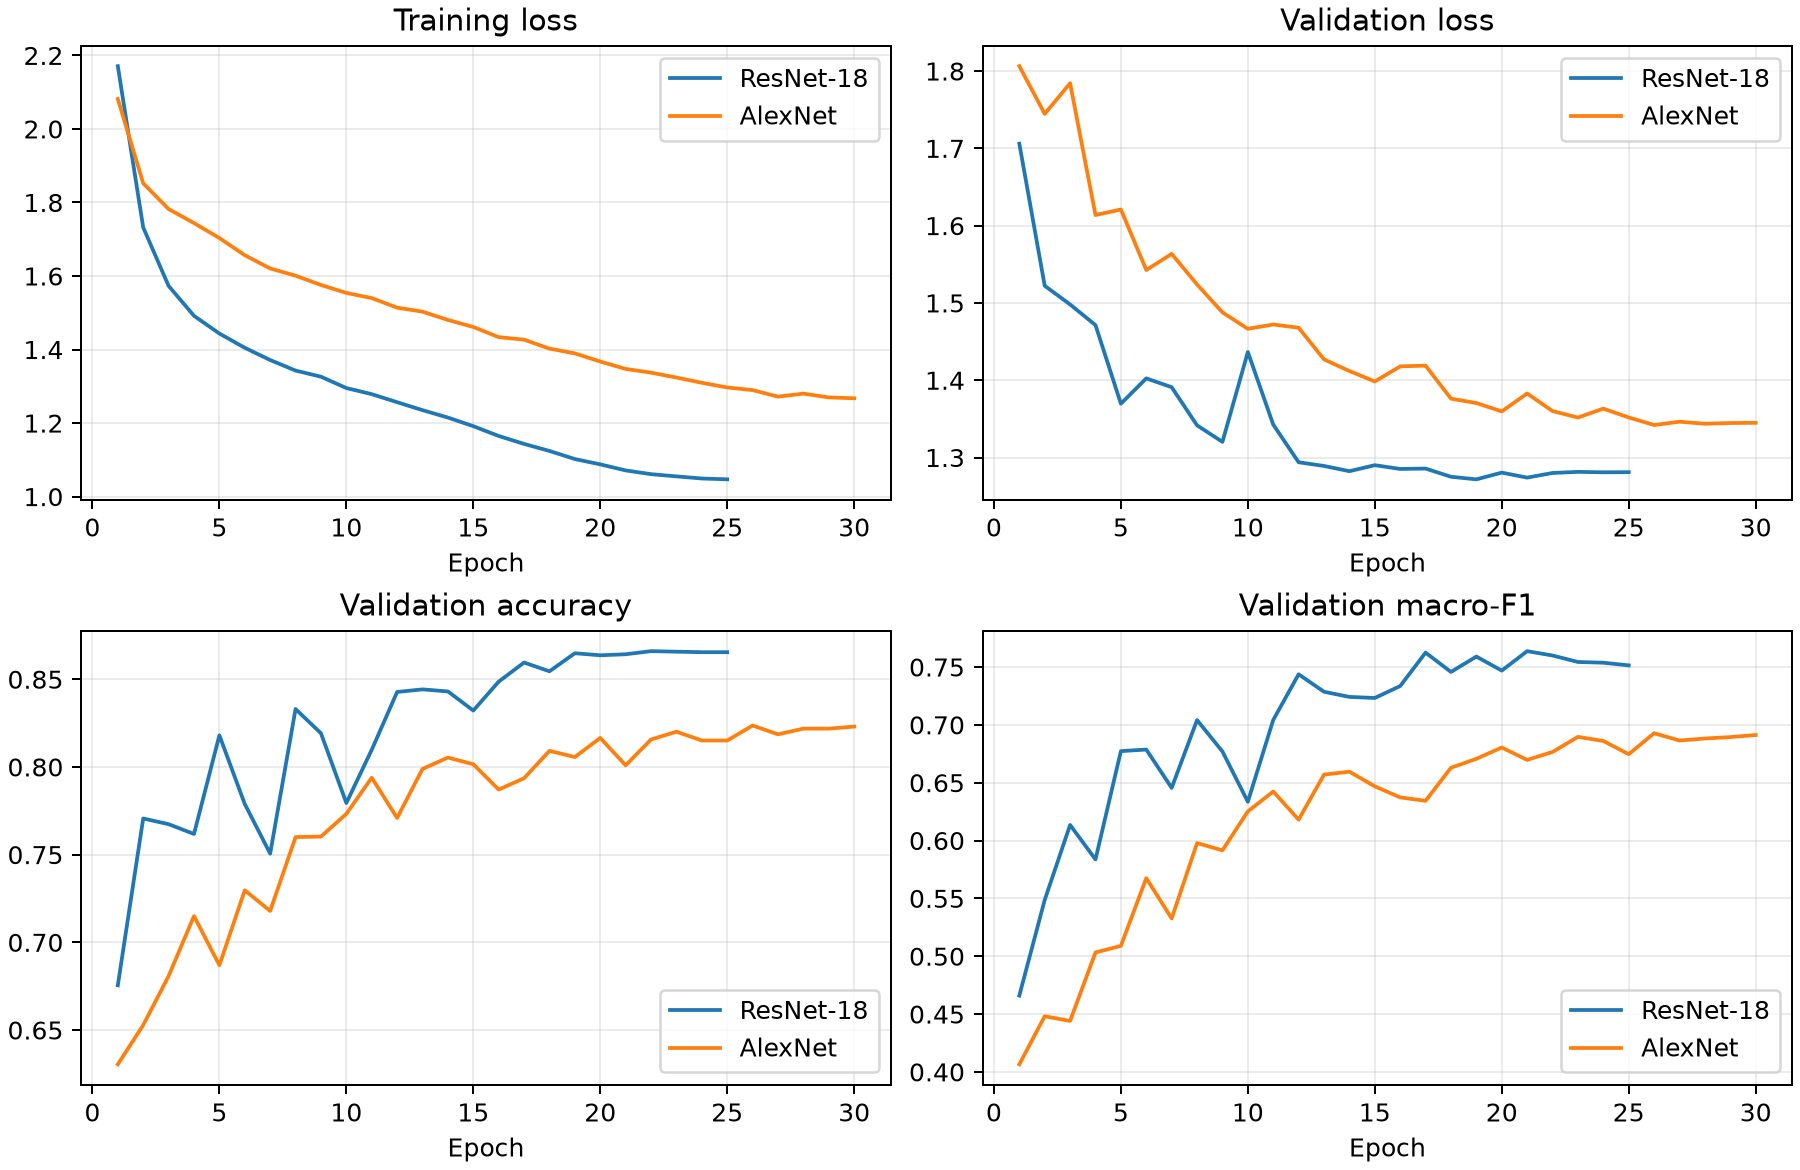
\includegraphics[width=0.97\textwidth]{results/resnet18_vs_alexnet.png}
\end{center}
\note{Figure 1. Training loss, validation loss, validation accuracy, and validation macro-F1. Loss is the weighted, smoothed cross-entropy used in both runs.}

{\small
\begin{tabularx}{\textwidth}{@{}rYrrrr@{}}
\toprule
Epoch & Model & Train loss & Val loss & Val accuracy & Val macro-F1\\
\midrule
1  & ResNet-18 & 2.171 & 1.706 & 67.6\% & 46.6\%\\
1  & AlexNet   & 2.081 & 1.806 & 63.0\% & 40.7\%\\
5  & ResNet-18 & 1.444 & 1.370 & 81.8\% & 67.7\%\\
5  & AlexNet   & 1.703 & 1.621 & 68.7\% & 50.9\%\\
25 & ResNet-18 & 1.047 & 1.281 & 86.5\% & 75.1\%\\
25 & AlexNet   & 1.297 & 1.352 & 81.5\% & 67.5\%\\
\bottomrule
\end{tabularx}\par}

ResNet-18 reduced the loss more quickly and sustained higher validation scores. AlexNet peaked at \metric{69.28} validation macro-F1 at epoch 26, compared with \metric{76.37} at epoch 21 for ResNet-18. Both validation losses levelled off while training losses continued to fall. On test, AlexNet trailed by \pp{4.08} macro-F1 and \pp{3.17} accuracy.

\href{https://arxiv.org/abs/1512.03385}{ResNet-18} uses residual connections and batch normalization, which can help fine-tune deeper features. \href{https://papers.neurips.cc/paper_files/paper/2012/file/c399862d3b9d6b76c8436e924a68c45b-Paper.pdf}{AlexNet} starts with an \sizepx{11} stride-4 convolution and downsamples early, which can discard subtle local features. Its 57.0 million parameters are concentrated in the fully connected classifier, versus 11.2 million for ResNet-18. The runs also differ in their 25- and 30-epoch OneCycle schedules.

\newpage
\section{Published accuracy references}

{\small
\begin{tabularx}{\textwidth}{@{}lYr@{}}
\toprule
Label protocol & Study and evaluation note & Reported score\\
\midrule
FER2013, 7 classes & \href{https://ietresearch.onlinelibrary.wiley.com/doi/full/10.1049/cdt2/1845378}{IET 12-layer CNN (2025)}, abstract maximum and happy-class score & 99.20\%\\
FER2013, 7 classes & \href{https://link.springer.com/article/10.1007/s10791-026-10715-8}{ResNet50--Transformer (2026)}, stated overall score & 89.70\%\\
FER2013, 7 classes & \href{https://www.mdpi.com/2078-2489/17/10/982}{Global--local ensemble (2026)}, 7,178-image folder test split & 76.51\%\\
FER2013, 7 classes & \href{https://pmc.ncbi.nlm.nih.gov/articles/PMC11511472/}{SFER-MDFAE (2024)} & 76.18\%\\
FER2013, 7 classes & \href{https://arxiv.org/abs/2105.03588}{VGG-based single model (2021)}, no extra training images & 73.28\%\\
FER+ & \href{https://link.springer.com/chapter/10.1007/978-981-96-5887-9_18}{PAtt-Lite comparison (2025)}, abstract score & 96.20\%\\
FER+, 8 classes & \href{https://link.springer.com/article/10.1007/s44443-026-00740-4}{FER-EMFormer (2026)} & 95.78\%\\
\bottomrule
\end{tabularx}\par}

The highest FER2013 headline number in the reviewed papers, \metric{99.20}, is also the happy-class score in Section 4.1. The paper separately reports \metric{98.20} as a class mean and applies a confidence filter in its detailed evaluation. The paper claiming \metric{89.70} overall describes at least 991 errors across seven confusion-matrix cells. That exceeds the roughly 370 errors compatible with \metric{89.70} on the 3,589-image official private partition.

The PAtt-Lite abstract also reports \metric{68.40} balanced accuracy, and its full protocol was unavailable in the public preview. FER-EMFormer uses \sizepx{224} inputs and MS-Celeb-1M pretraining. The workshop ensemble's \metric{87.23} can be placed alongside those FER+ results with differences in filtering and pretraining in mind. Seven-class FER2013 uses different labels and sample eligibility.

\section{Photo inference}

The ensemble had the highest validation macro-F1 (\metric{77.24}) and was selected for photo inference. OpenCV detected and cropped a face in each of the three photos. The top expression scores were neutral (\metric{73.0}), happy (\metric{72.9}), and neutral (\metric{75.5}). The public report records the scores. The original photos and visual predictions are kept local.

\section{Reproducibility}

The original runs used Python 3.12.16, PyTorch 2.11.0+cu128, torchvision 0.26.0+cu128, facenet-pytorch 2.6.0, and OpenCV 4.14.0 on an RTX 4090. The \href{https://github.com/FakeForest/AffectNet2013}{workshop repository} includes training and inference code, per-epoch histories, aggregate plots, and the test metrics for each configuration.

\end{document}
